\begin{figure}[!h]
 \centering
 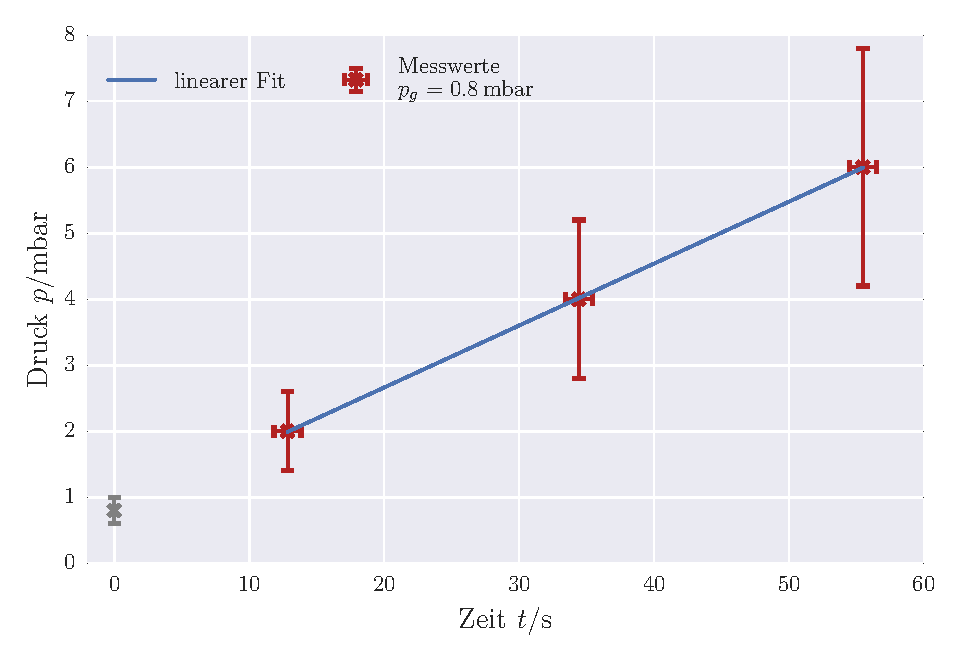
\includegraphics[scale=0.65]{../Grafiken/Leckrate_Drehschieber_3.pdf}
 \caption{Graphische Darstellung der Druckmesswerte in Abhängigkeit von der Zeit, aus der 4. Messreihe, und der
 entsprechenden Ausgleichsgeraden. Der für die Messreihe eingestellte Gleichgewichtsdruck ist angegeben und als Messwert für $t=0$ mit eingetragen. Dieser ist grau dargestellt, da er für die 
 Berechnung der Ausgleichsgeraden nicht verwendet wurde. Diese Auslassung wurde vorgenommen, da
 der tatsächliche Druck bei $t=0$, durch den plötzlichen Druckanstieg bei Schließung des Ventils zur Pumpe, von dem
 gemessenen Druck bei offenem Ventil abweicht. \label{fig:leckrate_drehschieber_3}}
 \end{figure} 